\documentclass[aspectratio=169,t,11pt,table]{beamer}
{\setbeamercovered{transparent}}
\usepackage{slides,math}
\usepackage{fontawesome}
\usepackage{textpos}
\usepackage{siunitx}
\usepackage{tikz}
\usetikzlibrary{positioning,arrows.meta,fit}
\usepackage{animate}
\usepackage{amssymb}
\usepackage{annotate-equations}

% Optionally define `accent`/`accent2` colors for theme customization
% I recommend changing the top slider on this: https://hslpicker.com/#1e9400
\definecolor{accent}{HTML}{940034}
\definecolor{accent2}{HTML}{006896}

\title{\huge Exploratory study of Neural Operators as surrogate models for collective effects in the FCC-ee High Energy Booster}
\date{\today}
\author{
  \texorpdfstring{
    \and Santiago~Martinez\inst{1}
  }{    Santiago Martinez
  }
}
\institute{
	\inst{1} GANIL/CNRS ;
}
\addbibresource{ref.bib}

\begin{document}

% ------------------------------------------------------------------------------
\begin{frame}[noframenumbering,plain]
\maketitle
\titlepage
\bottomright{
  \footnotesize M2 Internship\hspace{0.9cm}~

  \begin{tikzpicture}[remember picture,overlay]
    \node[yshift=-0.75cm, xshift=5.8cm] at (current page.north){%
      
\includegraphics[width=3cm]{figures/logo/LogoGANIL.png}};
  \end{tikzpicture}

  }
\end{frame}

% \begin{frame}[noframenumbering,plain]{Outline}
%   \vspace{-0.5cm}
%   \tableofcontents
% \end{frame}
% % ------------------------------------------------------------------------------

% ------------------------------------------------------------------------------
\section{Theoretical framework}
% ----------------------------------------------------------------------------



%------------------------------------------------------------------------------
\begin{frame}{Theoretical Framework}{Neural Operators \& Latent space decomposition}
  \vspace{-1cm}
  \begin{columns}[T]
    \begin{column}{.5\textwidth}
      \begin{purpleBlock}{\centering\small{Neural Operators as surrogate models for collective effects}}
        \[
          \frac{\partial \rho}{\partial s} + \{\rho,H\} = \mathcal{C}[\rho]
        \]
        Implies ($\mu$-parametrized) solution as 
        \[
            \rho_{s+\Delta s}=\mathcal{G}_\theta(\rho_s,\mu)\rho_s \approx e^{\Delta s \mathcal{L}_ {\mathrm{wake}}} e^{\Delta s \mathcal{L}_{\mathrm{ext}}}\rho_s.
        \]
        
      \end{purpleBlock}
         \end{column}
    \hfill
    \begin{column}{.5\textwidth}
      \begin{purpleBlock}{\centering\small{Surrogate for nonlinear effects}}
        \vspace{-0.2cm}
        \small
        In this context 
        \[
        e^{\Delta s \mathcal{L}_{\mathrm{ext}}}\in GL(\mathbb{R}^{N})   
        \]
        Is a linear operator, while
        \[
        e^{\Delta s \mathcal{L}_{\mathrm{wake}}}\in O(\mathbb{R}^{N})   
        \]
        Is a nonlinear operator. 
      \end{purpleBlock}
    \end{column}
  \end{columns}
 	
  
  \bottomleft{
  }
\end{frame}

%-------------------------
\begin{frame}{Theoretical Framework}{Neural Operators \& Latent space decomposition}
  \vspace{-1cm}
  \begin{columns}[T]
    \begin{column}{.5\textwidth}
        \begin{purpleBlock}{\centering\small{Latent space decomposition:}}
        \vspace{-0.2cm}
        \small
        Learning dynamics is performed in latent space of an Auto Encoder (AE)
        \[
          z = \mathcal{E}_\phi(\mathcal{H}(\rho),\,\sigma,\langle x\rangle)\in\mathbb{R}^{256},\ 
          \widehat{\mathcal{H}}(\rho)=\mathcal{D}_\psi(z).
        \]
        \vspace{0.1cm}

         The objective is $\; z_{t+1} = \mathcal{T}_\theta(z_t, \text{lattice}, \mu)\;$ and decode to phase-space projections.
      \end{purpleBlock}
      
         \end{column}
    \hfill
    \begin{column}{.5\textwidth}
      \begin{purpleBlock}{\centering\small{Neural Operators as surrogate models for collective effects}}
        \[
          \frac{\partial \rho}{\partial s} + \{\rho,H\} = \mathcal{C}[\rho]
        \]
        Implies ($\mu$-parametrized) solution as 
        \[
            \rho_{s+\Delta s}=\mathcal{G}_\theta(\rho_s,\mu)\rho_s \approx e^{\Delta s \mathcal{L}_ {\mathrm{wake}}} e^{\Delta s \mathcal{L}_{\mathrm{ext}}}\rho_s.
        \]
        
      \end{purpleBlock}
    \end{column}
  \end{columns}
 	
  
  \bottomleft{
  }
\end{frame}
%------------------------------------------------------------------------------

\begin{frame}{Theoretical Framework}{Data dimensionality reduction with a CVAE}
\vspace{-0.7cm}

\begin{columns}[T]

\begin{column}{0.5\textwidth}

\begin{purpleBlock}{\centering\small{Conditional Variational Auto Encoder}}

\tiny

The beam distribution is represented by 15 projected phase-space histograms

\[
x=\mathcal H(\rho)\in\mathbb R^{15\times64\times64},
\]

which are compressed into a probabilistic latent representation for some distribution $ \mathcal D(\mu_\phi,\Sigma_\phi)$

\[
q_\phi(z|x,a,d)
=
\mathcal D(\mu_\phi,\Sigma_\phi).
\]

The conditioning variables (beam moments and machine-domain parameters) are $ a=(\sigma,\langle x\rangle),\ d=(\mu,\kappa)$,
and provide sampling information for the latent space, 

\[
z=\mu+\exp\!\left(\frac12\log\sigma^2\right)\odot\epsilon,
\qquad
\epsilon\sim\mathcal N(0,I),
\]


\end{purpleBlock}

\end{column}

\hfill

\begin{column}{0.48\textwidth}

\begin{purpleBlock}{\centering\small{Encoder--Decoder}}

\tiny

Encoder

\[
(\mu,\log\sigma^2)
=
E_\phi(x,a,d)
\]

Decoder

\[
\hat x=D_\psi(z,d)
\]

The decoder reconstructs all 15 normalized phase-space projections simultaneously,

\[
\hat x
=
\widehat{\mathcal H}(\rho).
\]

The latent variable $ z\in\mathbb R^{256}$ provides a compact representation on which the neural operator performs time evolution.

\end{purpleBlock}

\end{column}

\end{columns}

\end{frame}

%-----------------------------------------------------------------------
\begin{frame}{Theoretical Framework}{Lattice Tokenization}

\vspace{-0.7cm}

\begin{columns}[T]

\begin{column}{0.5\textwidth}

\begin{purpleBlock}{\centering\small{Element embedding}}

\tiny

Each accelerator element is described by

\[
p_i=
(L,\theta,k_1,k_2,\ldots)
\in\mathbb R^7
\]

together with its longitudinal coordinate $s_i$.The normalized element parameters are embedded through a multilayer perceptron

\[
h_i^{(p)}
=
\mathrm{MLP}(p_i).
\]

This produces a learnable semantic representation of every lattice component.

\end{purpleBlock}

\end{column}

\hfill

\begin{column}{0.48\textwidth}

\begin{purpleBlock}{\centering\small{Fourier positional encoding}}

\tiny

Absolute position along the machine is encoded using multi-scale Fourier features

\[
\gamma(s)
=
\left[
\sin(\omega_ks),
\cos(\omega_ks)
\right]_{k=1}^{32},
\]

where fourier components are logarithmically spaced. The final token is

\[
h_i
=
\mathrm{MLP}(p_i)
+
W_p\gamma(s_i)
\in\mathbb R^{512}.
\]

This encoding captures both local optics and long-range machine periodicity.

\end{purpleBlock}

\end{column}

\end{columns}

\end{frame}

%-------------------------------------------------------------------
\section{Neural Operators}
%-------------------------------------------------------------------


\begin{frame}{Neural Operators}{Graph Neural Operator formulation}

\vspace{-0.7cm}
\begin{columns}[T]

\begin{column}{0.5\textwidth}
\begin{purpleBlock}{\centering\small{From PDEs to operator learning}}

\tiny

We consider a general elliptic PDE of the form

\[
\mathcal{L}_a u(x) = f(x), \quad x \in D,
\qquad
u(x) = 0, \quad x \in \partial D.
\]

For each coefficient field $a(x)$, the solution defines a mapping

\[
\mathcal{F}^{\text{true}}: a(\cdot) \mapsto u(\cdot).
\]

We aim to learn a discretization-invariant operator

\[
\mathcal{F}_\theta \approx \mathcal{F}^{\text{true}}
\quad \text{from samples } \{a_j, u_j\}.
\]

\end{purpleBlock}
\end{column}
\begin{column}{0.5\textwidth}
\begin{purpleBlock}{\centering\small{Green's function formalism}}

\tiny

The solution operator can be written as an integral operator

\[
u(x) = \int_D G_a(x,y)\, f(y)\, dy,
\]

where $G_a$ is the Green’s function depending on $a(x)$.

We replace it with a learnable kernel

\[
u(x)
=
\int_D \kappa_\theta(x,y,a(x),a(y))\, u(y)\, dy.
\]

This defines a data-driven Green’s function approximation.

\end{purpleBlock}
\end{column}
\end{columns}

\end{frame}


%---------------------------------------------------------------------

\begin{frame}{Neural Operators}{Iterative kernel evolution \& graph form}

\vspace{-0.7cm}
\begin{columns}[T]
\begin{column}{0.5\textwidth}
\begin{purpleBlock}{\centering\small{Iterative solver view}}

\tiny

Instead of solving directly the differential equation, we iterate:

\begin{align*}
         v_{t+1()}(x) & = \sigma\left(W v_t(x) + \right. \\
         & \left. \int_{B(x,r)} \kappa_\theta(x,y,a(x),a(y)) v_t(y)\, dy \right).
\end{align*}

This defines a nonlinear implicit propagation scheme over function space.

\end{purpleBlock}
\end{column}
\begin{column}{0.5\textwidth}
\begin{purpleBlock}{\centering\small{Graph discretization}}

\tiny

On a discretization $P_K = \{x_i\}_{i=1}^K$:

\begin{align*}
         v_{t+1()}(x) & = \sigma\left(W v_t(x) + \right. \\
         & \left. \frac{1}{|N(i)|} \sum_{j \in N(i)} \kappa_\theta(x_i,x_j,a_i,a_j)\, v_t(x_j) \right).
\end{align*}

This is equivalent to message passing on a graph with learned edge kernels that can be directed enforcing \textbf{causality}:

\[
m_{ij} = \kappa_\theta(e_{ij}) v_j,
\quad
e_{ij} = (x_i,x_j,a_i,a_j).
\]

\end{purpleBlock}
\end{column}
\end{columns}

\end{frame}
%---------------------------------------------------------------------
\begin{frame}{Baseline Model}{Latent-space Transformer tracking}

\vspace{-0.7cm}
\begin{columns}[T]
\begin{column}{0.5\textwidth}
\begin{purpleBlock}{\centering\small{Transformer formulation in latent space}}

\tiny

The baseline a standard autoregressive transformer operating on lattice tokens:

\begin{equation*}
    h_i = \mathrm{Tok}_\eta(p_i, s_i), \qquad h_i \in \mathbb{R}^{512}.
\end{equation*}
Latent evolution is modeled as:

\begin{equation*}
    z_{i+1} = \mathrm{Transformer}_\theta(z_i, h_{\le i}), \quad z_0 = \mathcal{E}_\phi(x,a,d).
\end{equation*}

This corresponds to:

\begin{equation*}
    z_N = z_0 + \sum_{i \le N} \Delta z_i,
\end{equation*}

with causal masking enforcing sequential dependence.

\end{purpleBlock}
\end{column}
\begin{column}{0.5\textwidth}
\begin{purpleBlock}{\centering\small{Features}}

\tiny

The attention mechanism is defined as:

\begin{equation*}
    \mathrm{A}(Q,K,V)=\mathrm{softmax}\left(\frac{QK^\top}{\sqrt{d}}\right)V.
\end{equation*}

it introduces key unphysical effects in the context of beam dynamics:
\begin{itemize}
\item global dense interactions (non-local mixing)
\item weak inductive bias for spatial structure
\item $O(N^2)$ complexity in lattice length
\end{itemize}

\end{purpleBlock}
\end{column}
\end{columns}

\end{frame}

%---------------------------------------------------------------------


\section{Architecture}
%-------------------------------------------------------------------

\begin{frame}{Architecture}{CVAE + GNO}

Proposed architecture
\begin{figure}
\centering
\resizebox{0.98\textwidth}{!}{
\begin{tikzpicture}[
  font=\small,
  box/.style={
    draw,
    rounded corners,
    align=center,
    inner sep=5pt,
    minimum height=10mm
  },
  arrow/.style={-Latex, thick},
  node distance=6mm and 6mm
]

\node[box] (rho) {6D beam snapshot\\$\rho$ (particles)};

\node[box, right=of rho] (hist) {15 pairwise\\projections\\$\mathcal{H}(\rho)\in\mathbb{R}^{15\times64\times64}$};

\node[box, right=of hist] (vaeenc) {VAE encoder\\$z_0=\mathcal{E}_\phi(\mathcal{H}_0,\sigma_0,\langle x\rangle_0)$\\$z_0\in\mathbb{R}^{256}$};



\node[box, right=of vaeenc] (gno) {Causal GNO in latent space\\$\Delta z_i = \mathcal{K}_\theta(z_0,h_{1:i},\mu)$\\$z_i=z_0+\sum_{k\le i}\Delta z_k$};

\node[box, below=of gno] (token) {Lattice tokenization\\$h_i=\mathrm{Tok}_\eta(p_i,s_i)$\\$h_i\in\mathbb{R}^{512}$};

\node[box, right=of gno] (vaedec) {VAE decoder\\$\widehat{\mathcal{H}}_N=\mathcal{D}_\psi(z_N)$};

\node[box, right=of vaedec] (loss) {Loss\\$\|\widehat{\mathcal{H}}_N-\mathcal{H}_N\|^2$\\$+\ \lambda\,\mathcal{L}_{mom}+\beta\,KL$};

\draw[arrow] (rho) -- (hist);
\draw[arrow] (hist) -- (vaeenc);
\draw[arrow] (vaeenc) -- (gno);
\draw[arrow] (token) -- (gno);
\draw[arrow] (gno) -- (vaedec);
\draw[arrow] (vaedec) -- (loss);

\node[box, left=of token] (lat) {Lattice elements\\$\{p_i, \mu_i, s_i\}_{i=1}^N$};
\draw[arrow] (lat) -- (token);

\end{tikzpicture}
}
\vspace{0.5cm}
%\caption{\small Proposed surrogate: VAE compresses 15 projected marginals; a causal graph neural operator propagates the latent along the lattice; decoder reconstructs 2D projections for supervision.}
\end{figure}
\bottomleft{\tiny{\textit{Training data was generated using X-suite and PyHEADTAIL including CST data as the impedance model.}}}
\end{frame}
%--------
\begin{frame}{Architecture}{Graph Neural Operator configuration}
\begin{purpleBlock}{\centering\small{Graph Neural Operator configuration}}

\scriptsize

\begin{tabular}{ll}
Hidden width & 512 \\
Operator layers & 4 \\
Token dimension & 512 \\
Element parameters & 7 \\
Fourier frequencies & 32 pairs (64 features) \\
Activation & GELU \\
Propagation & Kernel message passing \\
Tracking & Non-autoregressive \\
\end{tabular}

\end{purpleBlock}
\end{frame}
%-----

\begin{frame}{Architecture}{Optimization objective}

\vspace{-0.7cm}

\begin{columns}[T]

%-------------------------------------------------
\begin{column}{0.50\textwidth}

\begin{purpleBlock}{\centering\small{Total objective}}

\tiny

The model is trained using a multi-objective loss

\[
\boxed{
\mathcal L =
\mathcal L_{\rm hist}
+
\lambda_\sigma \mathcal L_\sigma
+
\lambda_c \mathcal L_{\rm cent}
+
\beta \mathcal L_{\rm KL}
}
\]

where

\[
\mathcal L_{\rm hist}
=
\left\|
\widehat{\mathcal H}_N-
\mathcal H_N
\right\|_2^2,
\]

\[
\mathcal L_\sigma
=
\left\|
\widehat{\log\sigma}
-
\log\sigma
\right\|_2^2,
\]

\[
\mathcal L_{\rm cent}
=
\left\|
\hat c-c
\right\|_2^2.
\]

The reconstruction loss is evaluated on normalized
15-channel pairwise beam projections.

\end{purpleBlock}

\end{column}

%-------------------------------------------------
\begin{column}{0.48\textwidth}

\begin{purpleBlock}{\centering\small{KL regularization}}

\tiny

The latent posterior is constrained towards a unit Gaussian,

\[
\mathcal L_{\rm KL}
=
\frac12
\sum_i
\left(
e^{\log\sigma_i^2}
+
\mu_i^2
-
1
-
\log\sigma_i^2
\right).
\]

Provides the follwing properties: 
\begin{itemize}
\item regularize the latent distribution;
\item promote a smooth and continuous latent manifold;
\item prevent overfitting and posterior collapse;
\item improve interpolation and extrapolation;
\item provide a stable latent space for the downstream GNO evolution.
\end{itemize}

\end{purpleBlock}

\end{column}

\end{columns}

\end{frame}
%--------------------------------------------------------------------

\section{Preliminary Results}
%-------------------------------------------------------------------
\begin{frame}{Preliminary Results}{CVAE latent space reconstruction}
\vspace{-0.2cm}

\begin{figure}
    \centering
    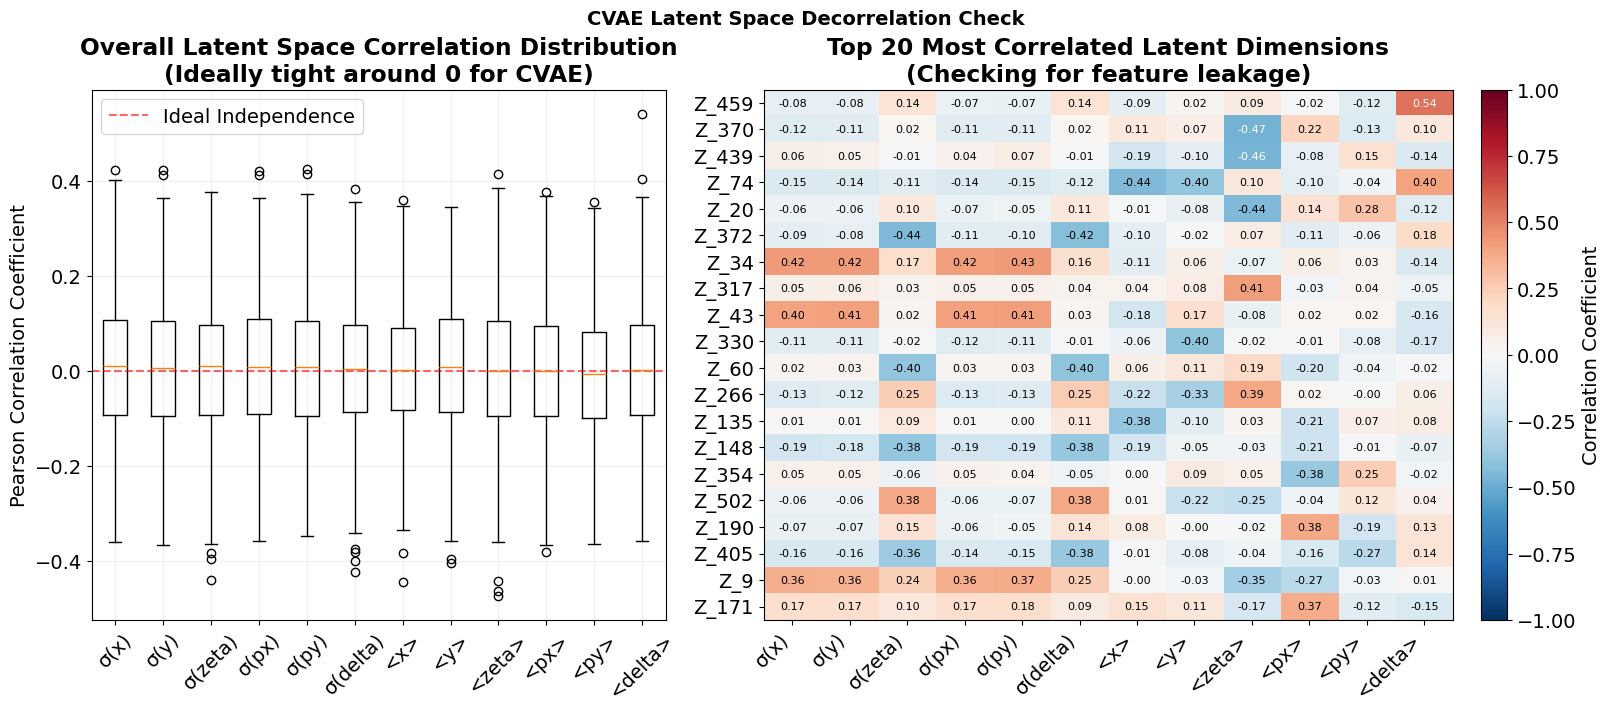
\includegraphics[width=\linewidth]{figures/corr_VAE.png}
\end{figure}

\end{frame}
%---------






%--------




\begin{frame}{Preliminary Results}{CVAE latent space reconstruction}
\vspace{-0.7cm}

\begin{purpleBlock}{\centering\small{Key observations}}
\small

\begin{itemize}

\item Global latent–physics correlation is close to zero across almost all dimensions.

\vspace{0.2cm}

\item The distribution is sharply centered around 0, indicating weak linear dependence between latent variables and physical summaries.

\vspace{0.2cm}

\item Only a small subset of latent dimensions shows moderate correlation ($\sim 0.3$–$0.4$).

\vspace{0.2cm}

\item These correlated modes are sparse and not structurally organized.

\vspace{0.2cm}

\item No systematic leakage of physical variables into the latent representation is observed.

\end{itemize}

\end{purpleBlock}

\end{frame}
%---------
\begin{frame}{Preliminary Results}{GNO vs Transformer latent space dynamics}
\vspace{-0.2cm}

\begin{figure}
    \centering
    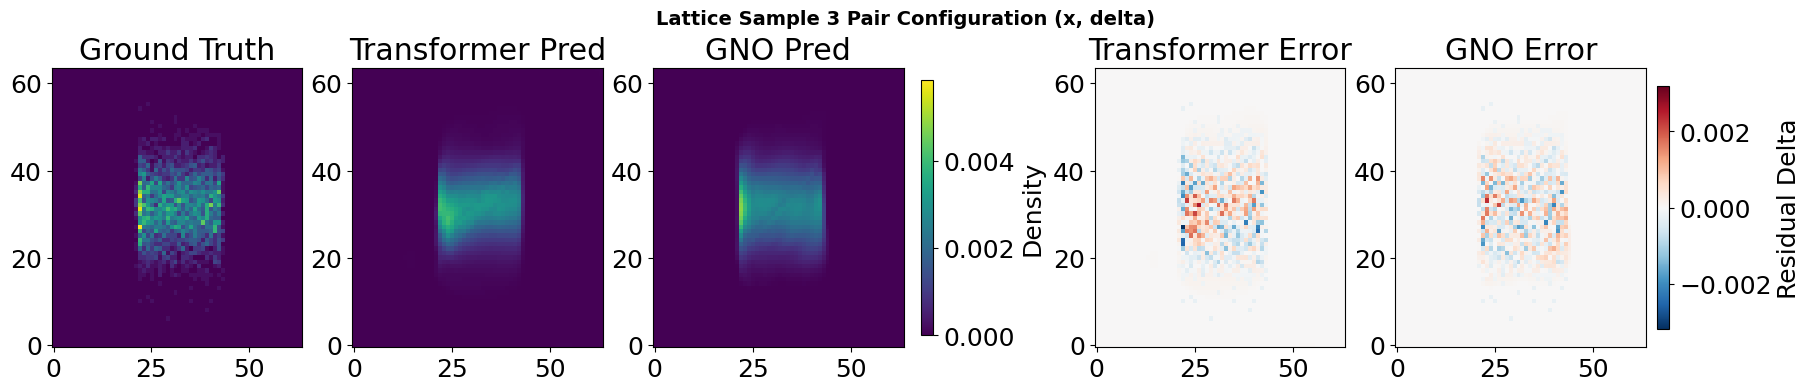
\includegraphics[width=\linewidth]{figures/GNO_VAE_1.png}
\end{figure}

\end{frame}
%---------
\begin{frame}{Preliminary Results}{GNO vs Transformer latent space dynamics}
\vspace{-0.2cm}

\begin{figure}
    \centering
    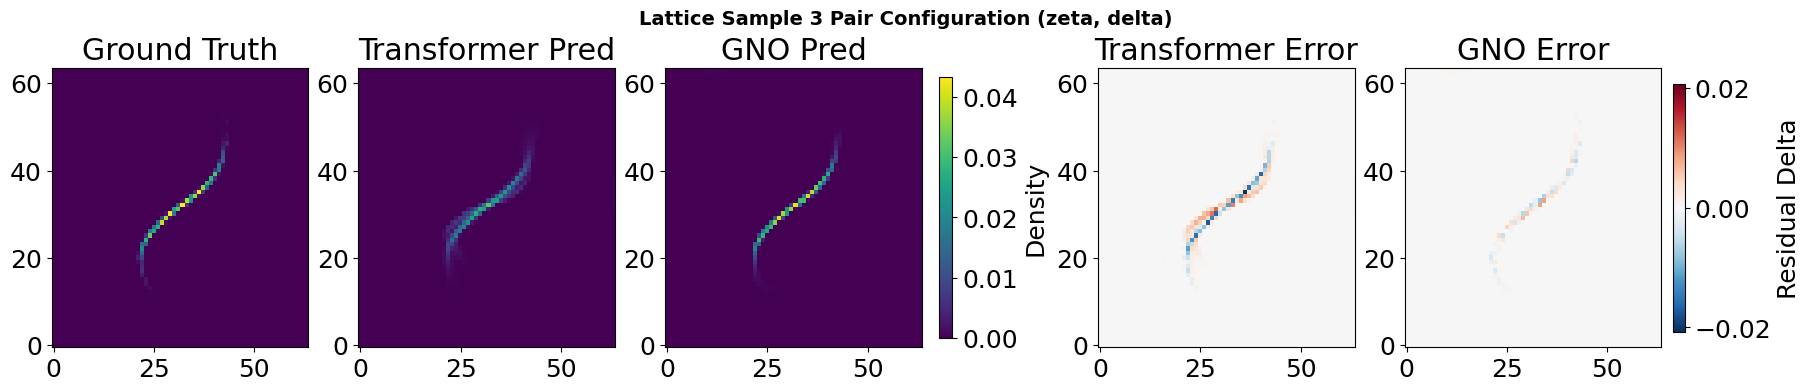
\includegraphics[width=\linewidth]{figures/GNO_VAE_2.png}
\end{figure}

\end{frame}

%---------
\begin{frame}{Preliminary Results}{GNO vs Transformer latent space dynamics}
\vspace{-0.2cm}

\begin{figure}
    \centering
    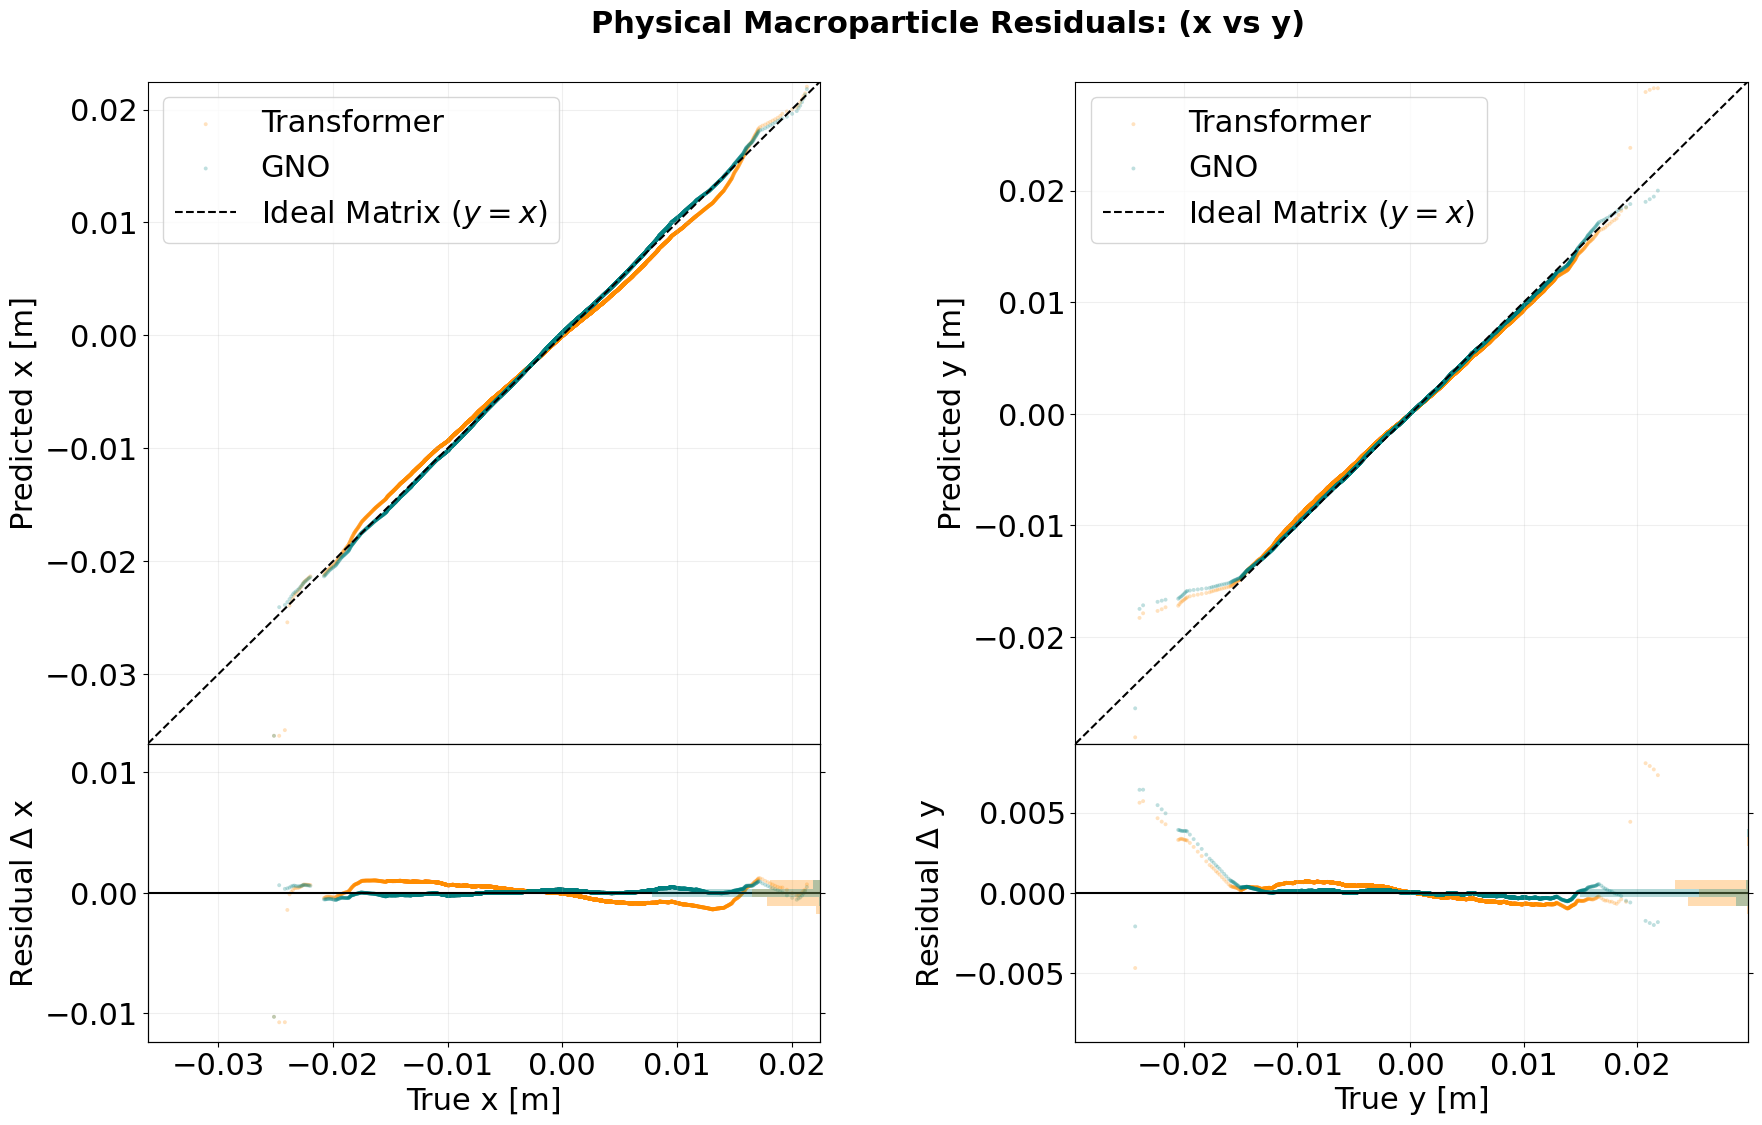
\includegraphics[width=0.6\linewidth]{figures/GNO_VAE_3.png}
\end{figure}

\end{frame}

%---------
\begin{frame}{Preliminary Results}{GNO vs Transformer latent space dynamics}
\vspace{-0.2cm}

\begin{figure}
    \centering
    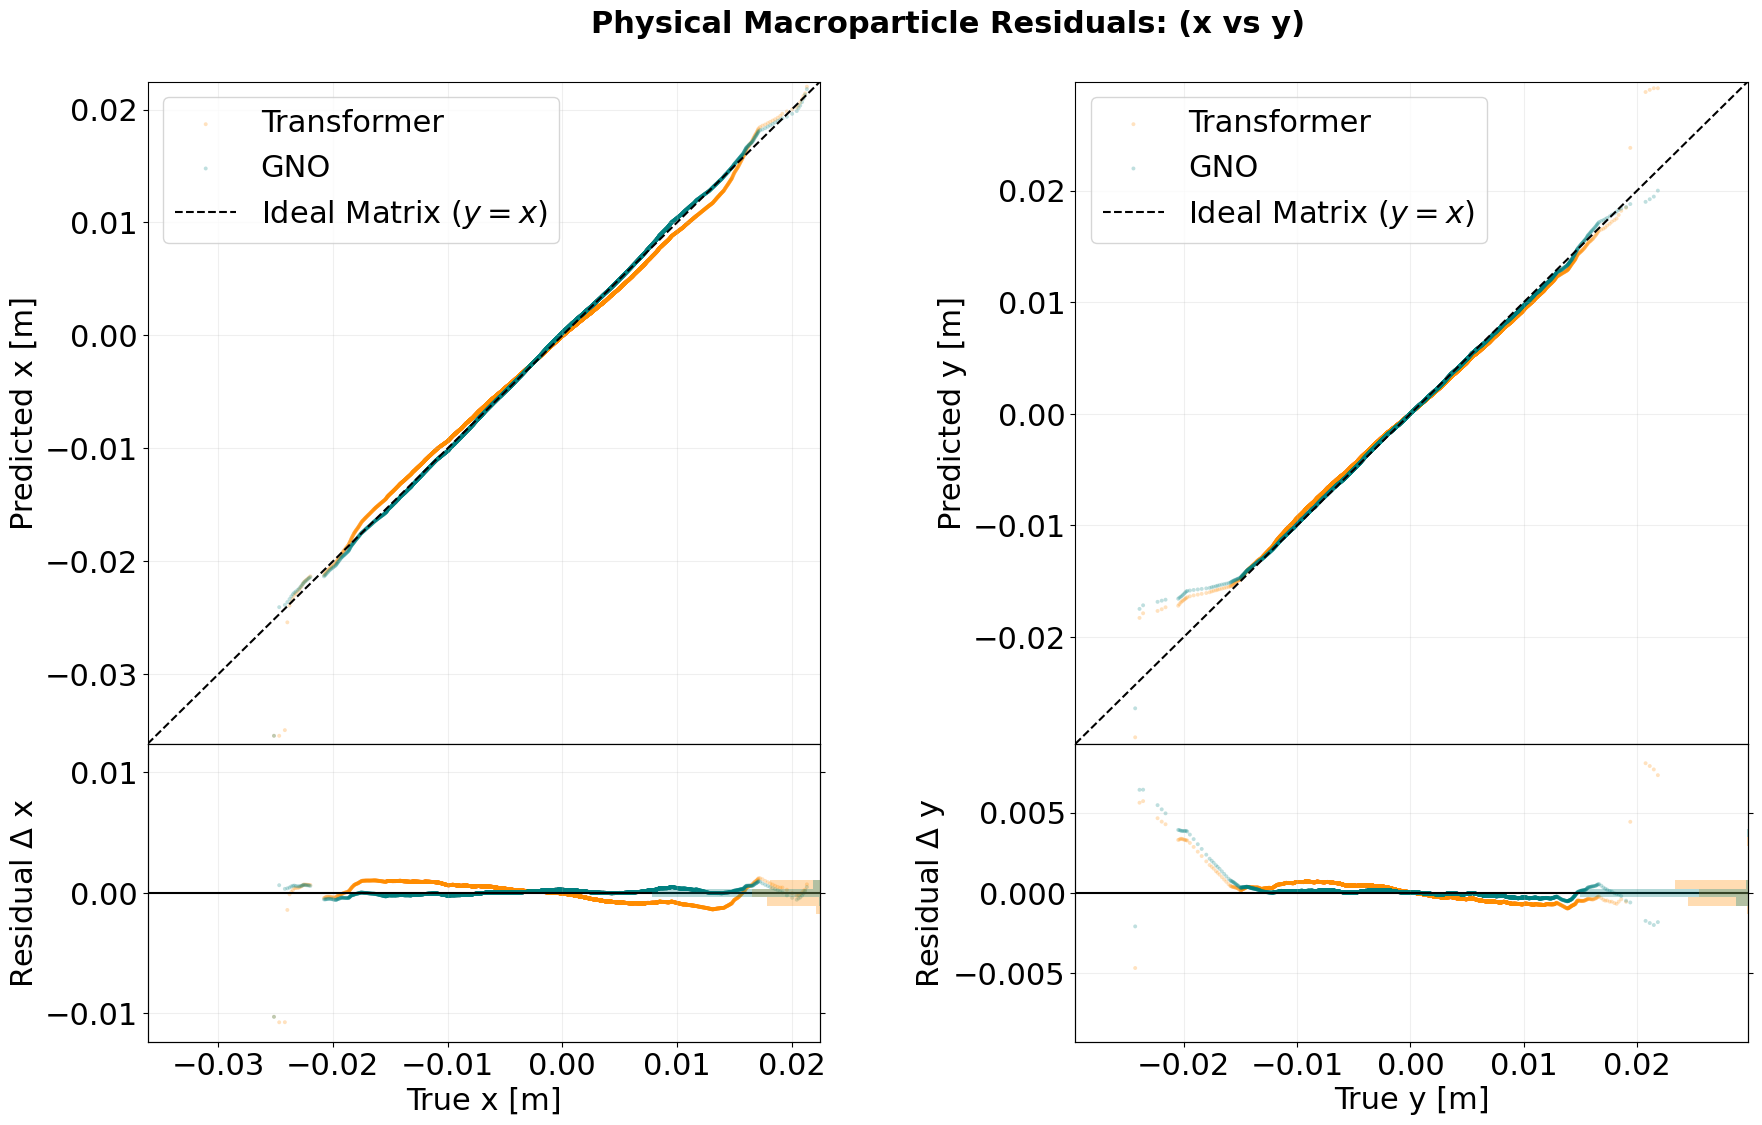
\includegraphics[width = 0.6\linewidth]{figures/GNO_VAE_4.png}
\end{figure}

\end{frame}
%--------------`'
\begin{frame}{Preliminary Results}{GNO vs Transformer latent space dynamics}
    GNO marginals exhibit causality
\vspace{-0.2cm}

\begin{figure}
    \centering
    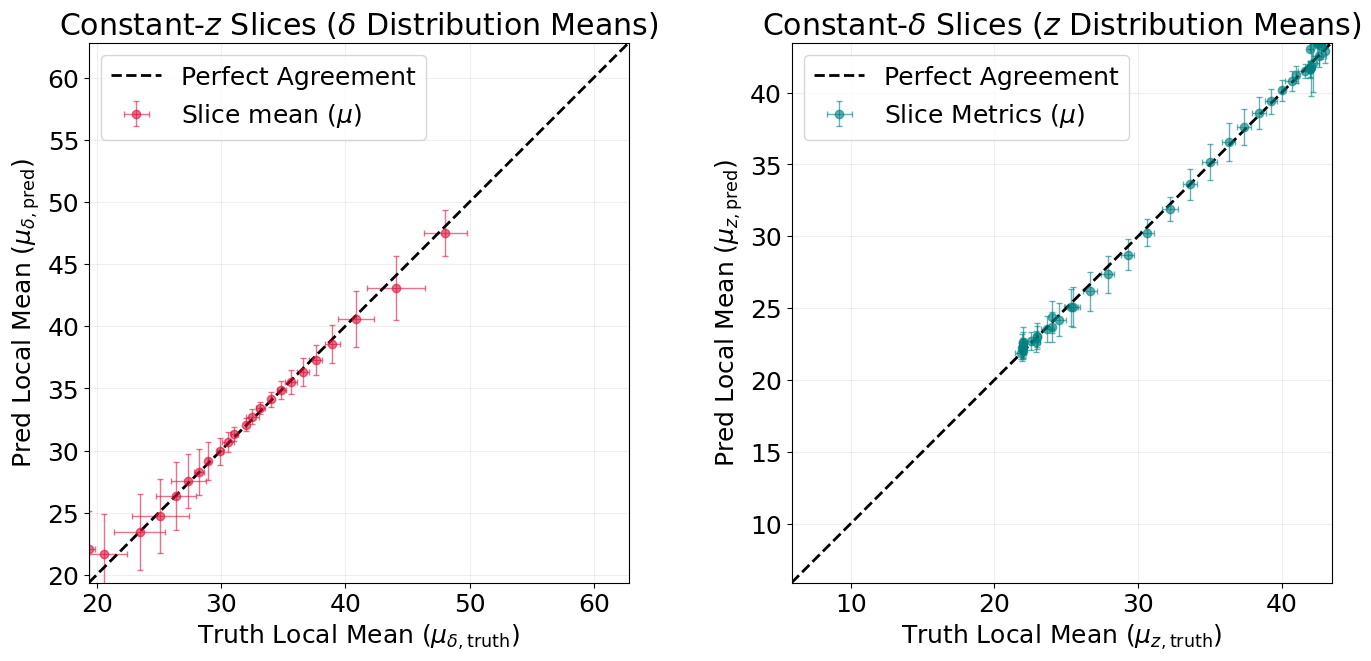
\includegraphics[width = 0.6\linewidth]{figures/GNO_marginals.png}
\end{figure}

\end{frame}
%--------------`'
\begin{frame}{Preliminary Results}{GNO vs Transformer latent space dynamics}
   Transformer marginals may produce artifacts due to non-causal attention
\vspace{-0.2cm}

\begin{figure}
    \centering
    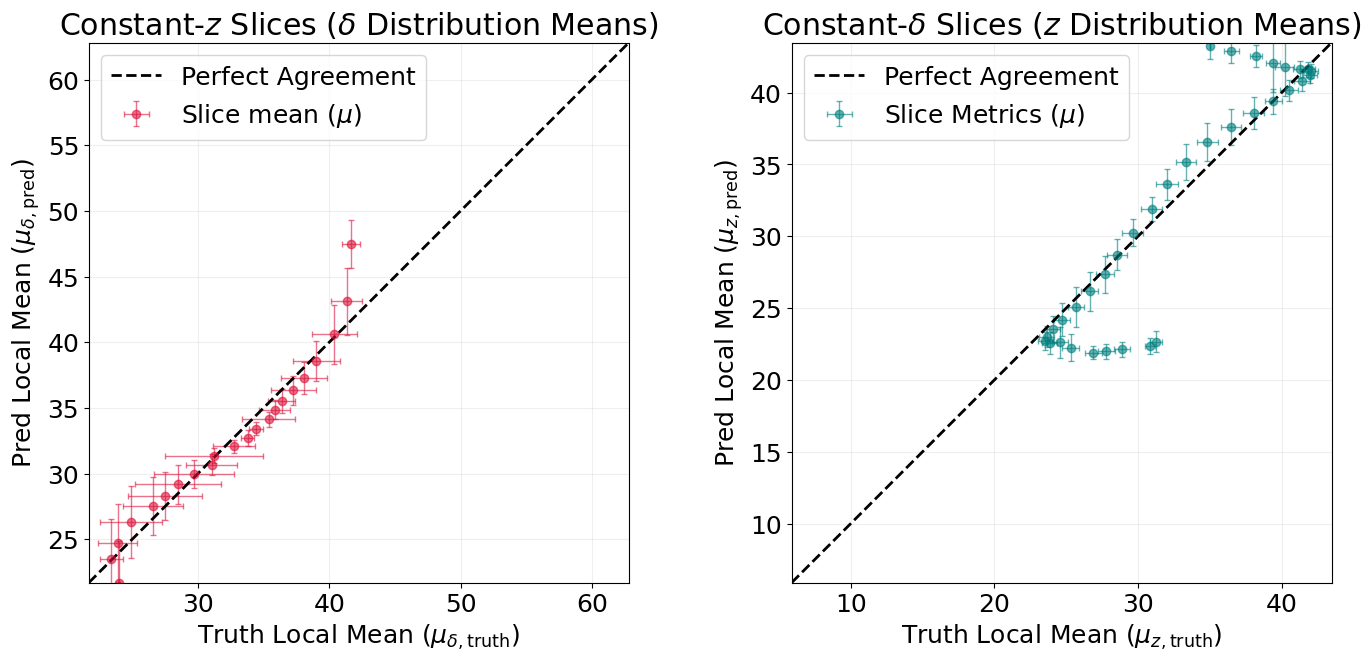
\includegraphics[width = 0.6\linewidth]{figures/TF_marginals.png}
\end{figure}

\end{frame}

\begin{frame}{}{}
   
\vspace{-0.2cm}

\begin{figure}
    \centering
    
\includegraphics[width = 0.6\linewidth]{figures/gracias.jpg}
\end{figure}

\end{frame}


\end{document}
%This work was granted access to the HPC resources of IDRIS under the allocation 2024-103810 made by GENCI